\documentclass{article}
\usepackage[utf8]{inputenc}
\usepackage{indentfirst}
\usepackage[final]{graphicx}
\usepackage{subcaption}
\usepackage{psfrag,amsbsy,graphics,float}
%\usepackage[pdftex]{graphicx, color}

\usepackage{amsmath}
\DeclareMathOperator*{\argmax}{arg\,max}
\usepackage{gensymb}

\setlength{\parskip}{1em}


\title{\Huge{Poppy Intermediate Report}}
\author{M. Fares Abid \\ Bo Huang \\ Maxime Kirgo \\ Dominik Meinzer \\ Rémi Laumont }
\date{\textit{Lehrstuhl für Datenverarbeitung} \\ \textit{Technische Universität München} \\ \textbf{June $22^{nd}$ 2017}}

\begin{document}

\maketitle



\section{Introduction}

Our project is a basic robotic problem and aims to make the humanoid robot Poppy learn motion control. This means that we want it to learn how to control its arm to a given target position. Although there already exist some techniques such as inverse kinematics (IK) to generate motion, they have drawbacks like special treatment of singularities and joint limitations. For this reason we use deep Q-learning to learn a simple reaching task. In detail, we use the \textit{Deep Q-Network} algorithm, proposed by Mnih et al. \cite{mnih_human, mnih_play} and including the ideas of a replay memory and a target network.

\vspace{\baselineskip}

In addition, we introduce our own exploration policy, because $\epsilon$ -greedy is not suitable for exploration in robotics and does not result in a short learning time. The exploration is based on an IK approach to guide the robot arm in the direction of the target and explore randomly around this trajectory. 

\section{Modeling}

\subsection{Markov Decision Process}
Due to the short project time, we use a simplified version of the problem. Consequently, we focus on motion of one arm of the robot. Additionally, we decrease the degrees of freedom of the Poppy arm from 4 to 2, see Fig. \ref{fig:poppy_2dof}. This means that we are restricting the control to motors \textit{$l\_shoulder\_x$} and \textit{$l\_elbow\_y$}, called in the following $\theta_1$ and $\theta_2$ respectively. Motor $l\_shoulder\_y$ is set to $-90\degree$ and motor $l\_arm\_z$ is hold at $0\degree$ in order to allow movements of the hand only in the x-axis (sideways) and y-axis (forward/backwards).

\vspace{\baselineskip}

The state space is a description of the robot and the environment in only 4 states. We decided to reduce the state-space because we realized that the information was redundant and we noticed the enormous size of our state space, which has (discretized) at least $(200*150)^2$ states: $\theta_1$ and $\theta_2$ have respectively 200 and 150 possible angle positions, given a discretization of $1\degree$ each, to which we have to add the same dimensionality for the position of the goal, when sampling the goal only at possible angle configurations and not completely randomly. Consequently, we substituted the position of the end-effector and the position of the goal for the difference between the end-effector position in the x-y plane $\vec{x}_{arm} = [x_{arm}, y_{arm}]$ and the goal position in the x-y plane $\vec{x}_{goal} = [x_{goal}, y_{goal}]$:
\begin{equation}
\Delta \vec{x} = \vec{x}_{goal} - \vec{x}_{arm}
\end{equation}
but still use the two joint angles of the robot arm $\vec{\theta} = [\theta_1, \theta_2]$. The combination of these states also fulfill the Markov Property, but reduce the state space, where the state $s$ is given by:
\begin{equation}
s = [\Delta x, \Delta y, \theta_1, \theta_2]
\end{equation} 
where the arm joint angles $\theta_i$ and the position of the end-effector can be measured by the internal sensors of the robot. The goal position is still set by ourselves manually at the beginning of each episode. However, we are currently working on including vision in order to detect the goal position.
\\
Regarding the action space and the reward signal, we have not changed our initial design. The action space in our project is still 4 discrete actions. The agent controls two motors and can move each motor up and down with $\pm1\degree$. 
The reward $r$ is the negative distance between the end-effector position and the goal position:
\begin{equation}
r = -\left\Vert\left( \vec{x}_{arm} - \vec{x}_{goal} \right) \right\Vert^2
\end{equation}

\begin{figure}
	\centering
	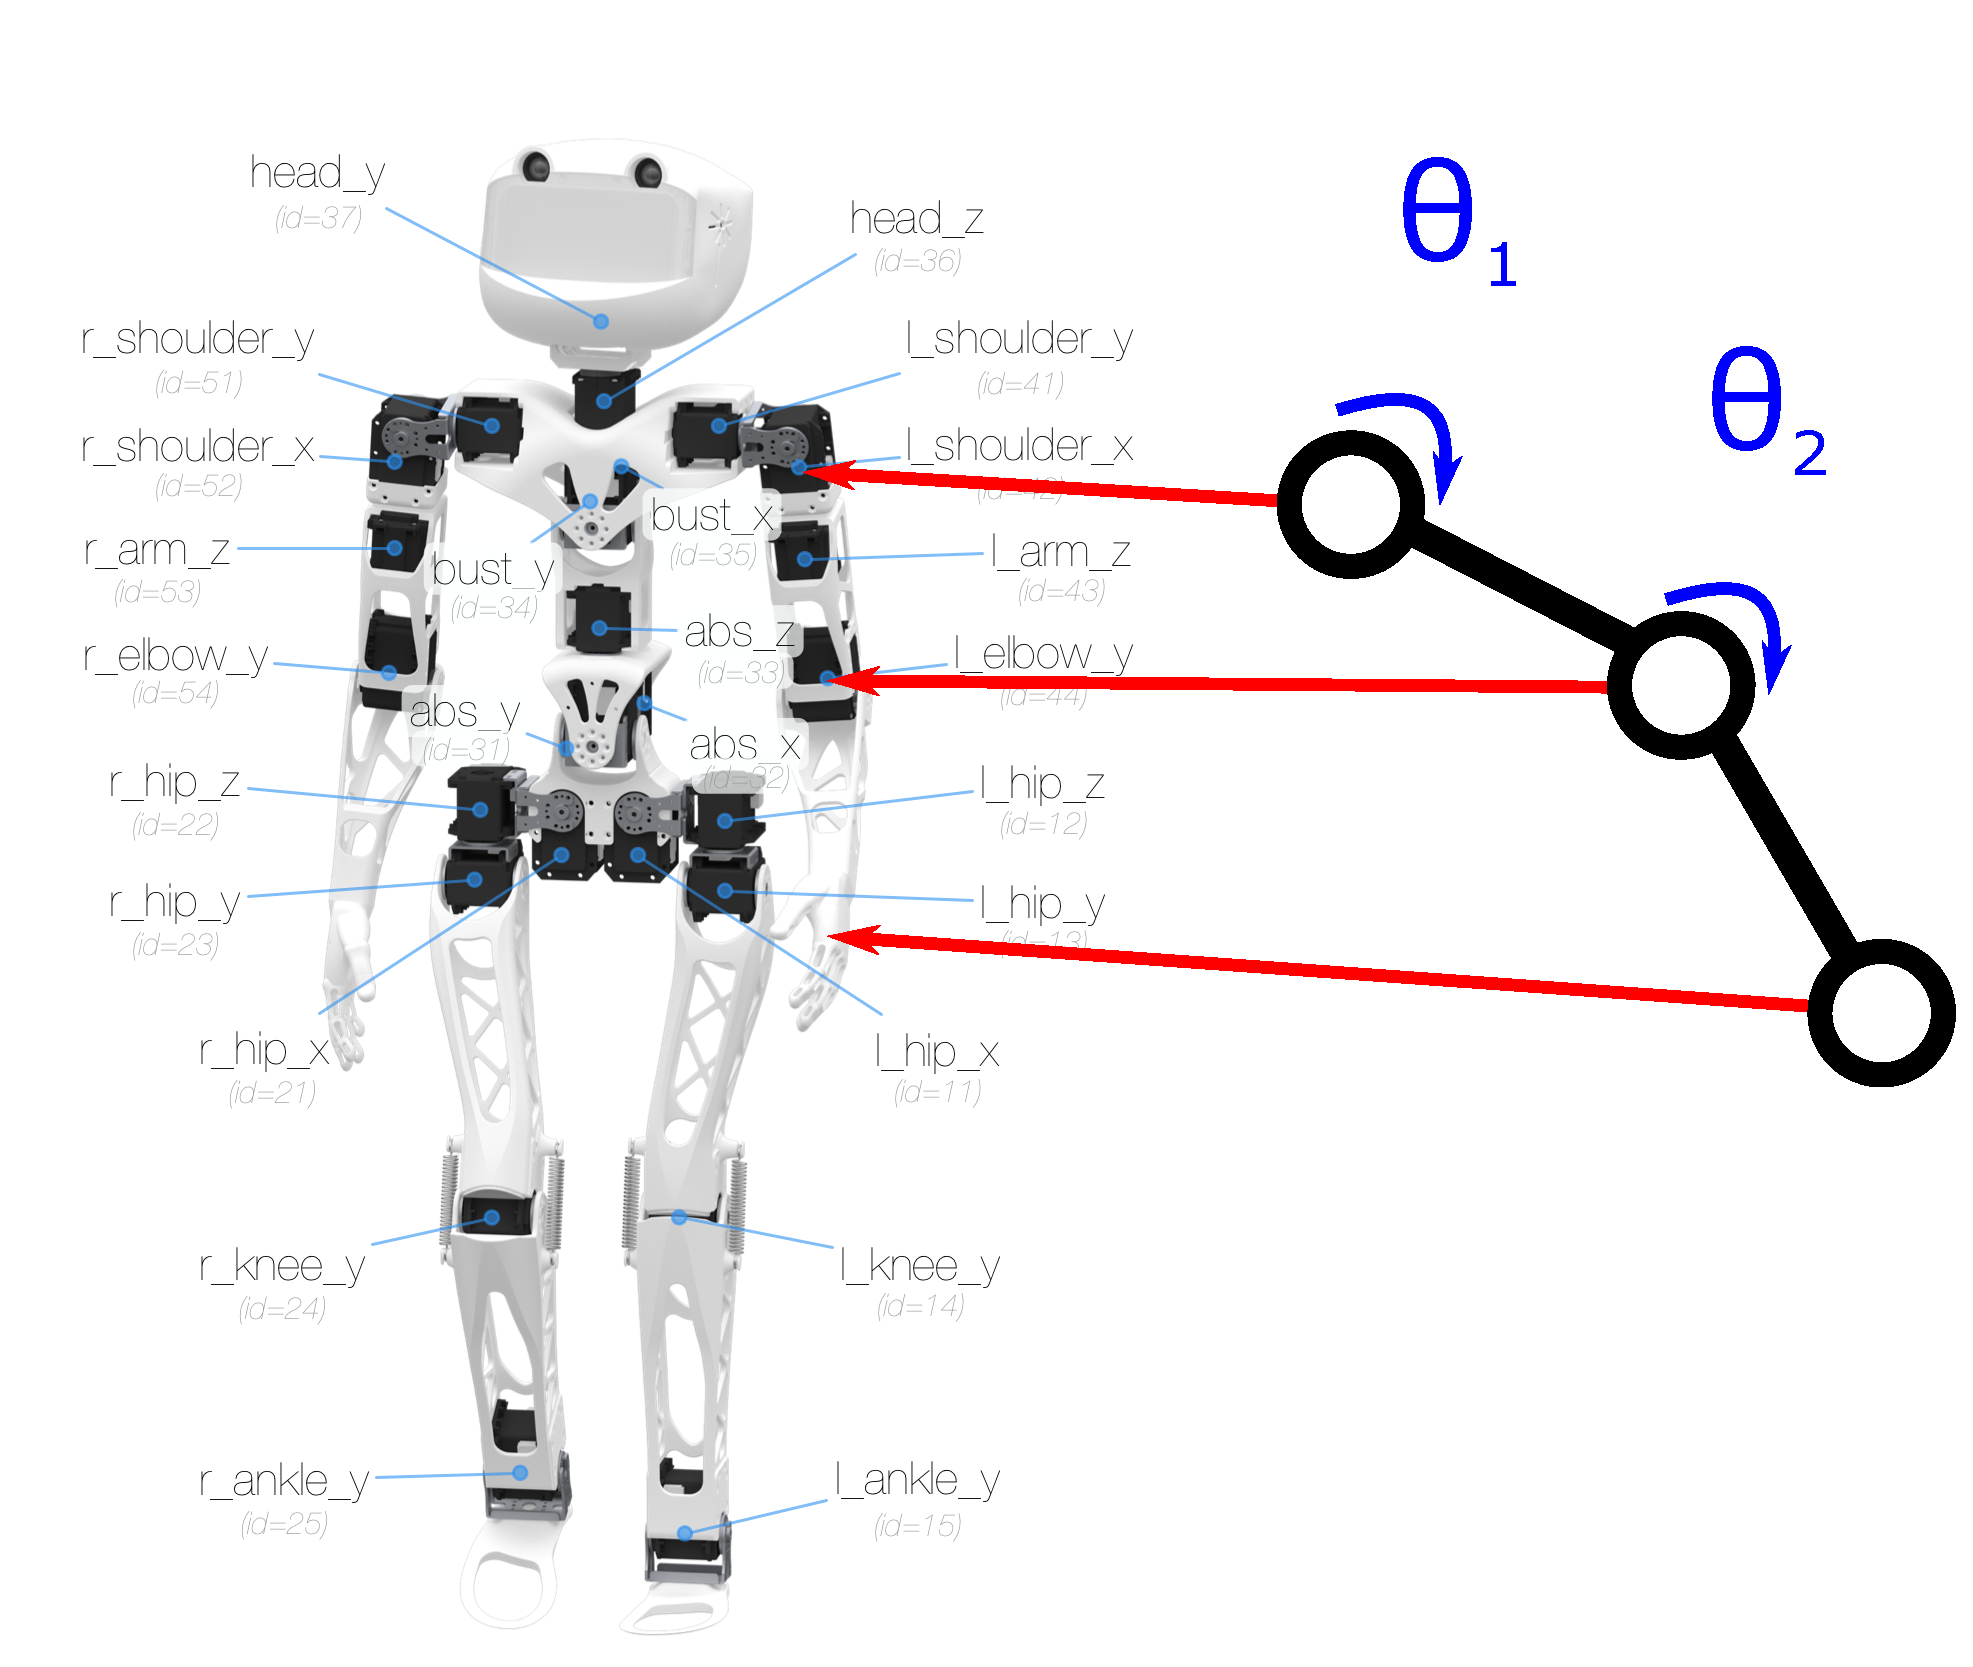
\includegraphics[width=0.7\textwidth]{reportpics/poppy_2dof.eps}
	\caption{Arm Modeling of Poppy}
	\label{fig:poppy_2dof}
\end{figure}

\subsection{Deep Q-Network}
The Q-Network has the same structure as at the beginning. This means that we are using 100 neurons with ReLU activation function for the input and the two hidden layers and 4 neurons with linear activation function for the output layer. The loss is the Mean-Squared Error (MSE) and the optimizer RMSprop. We also included normalization of the state space for neural network learning, because our $\theta$ is in rad or degrees and our positions in meters or centimeters. Consequently, we need to normalize each value to be between -1 and 1 in order to ensure a good problem conditioning.

\vspace{\baselineskip}

Regarding hyperparameters we had to tune the exploration parameter $\epsilon$ and the discount factor $\gamma$. Often a high $\gamma$ is preferred in order to have a far-sighted agent. Therefore, we started with $\gamma=0.9$, but the Q-values regularly diverged. Then, we lowered $\gamma$ to be finally $0.5$ and got convergence. Based on empirical studied, we assume that even though we have a non-linear function approximator the contraction using a low $\gamma$ is better. Furthermore, exploration based on just $\epsilon$-greedy did indeed not result in good policies after a short learning period. However, our own exploration policy based on IK lead to fast learning agents. The main idea of this guidance is to show the robot almost correct actions and to let the agent improve itself around this guidance by randomly selecting other actions. This means that with a probability of $\frac{\epsilon}{2}$ we take a random action and with probability $\frac{\epsilon}{2}$ we use the best action provided by the IK guidance. Otherwise, with a probability of $1-\epsilon$, we are not using exploration and follow the best action proposed by the Q-Network. The IK guidance is done in the following way. The joint angle velocities $\Delta \vec{\theta}$ are computed by:
\begin{equation}
\Delta \vec{\theta} = J^{-1} \cdot (\vec{x}_{goal} - \vec{x}_{arm})
\end{equation}
where $J$ is the Jacobian matrix of the robot arm at joint angles $\vec{\theta}$.\\
Then, the motor to control is determined by selecting the motor with the larger joint angle velocity:
\begin{equation}
\argmax_{i \in \{1,2\}}(\Delta \theta_1, \Delta \theta_2)
\end{equation}
Finally, the action is determined by the motor $i$ and the sign of the respective $\Delta \theta_i$ in order to decide the direction $\pm1\degree$. During training, $\epsilon$ is decreasing over the number of episodes, starting with $\epsilon_0 = 0.99$ and ending with $\epsilon_{min} = 0.05$. In between $\epsilon$ is defined by:
\begin{equation}
\epsilon_{i+1} = \frac{\epsilon_{i}}{1 + i \cdot eps_{decay}} 
\end{equation}
where $eps_{decay}$ is the rate of the exploration decay and $i$ is the number of the episode.
\\
In the beginning, we used a fast decreasing epsilon ($eps_{decay}=0.00005$), but had to restart training 2 or more times in order to get a good policy. We noticed that the agent has to try more random and guided actions to achieve a better policy. Fig.~\ref{fig:epsilon} shows the previous epsilon over episodes and the current (using $eps_{decay}=0.000001$). First experiments show indeed faster learning.
\begin{figure}
	\centering
	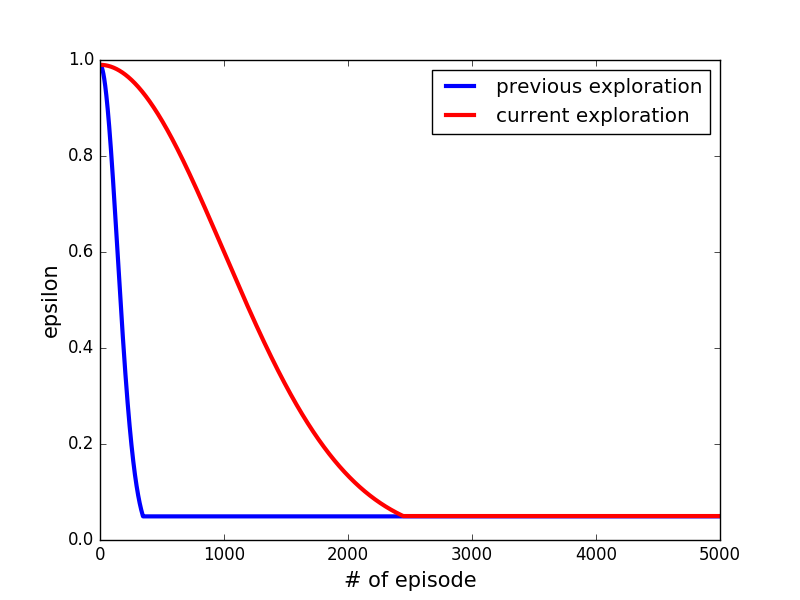
\includegraphics[width=0.7\textwidth]{reportpics/epsilon.png}
	\caption{Exploration over episodes. }
	\label{fig:epsilon}
\end{figure}


\section{Proof of Concept}
First, we tried to set up the simulation of Poppy in V-Rep, but we realized very fast that simulation noise and numerical error result in different behavior of the same code on different PCs. Therefore, we decided to train in a simplified self-built fully deterministic simulation. The simulation approximates the Poppy arm as a 2-DOF robot arm with upper arm length 15.1~cm and lower arm length 10.1~cm, disrespecting small offsets in the two motor axes. The robot arm simulation can be seen in Figs. \ref{fig:scenario1} and \ref{fig:scenario2}. \\
During the training phase, the robot arm is initialized with $\vec{\theta} = [0,0]$ at the beginning of the first episode and left unchanged after every episode. The goal positions are sampled uniform randomly from the possible robot arm angle configurations in order to sample a goal inside the joint limits. The maximum number of timesteps per episode is 500. If the goal is reached before 500 steps, i.e. the different between end-effector position and goal position is less than the threshold of 0.5~cm, or the 500 steps have passed, a new goal position is initialized. Collecting training samples is performed in 8 parallel threads in order to sample from distinct environments at the same time. Before changing the exploration parameter, we needed 2 or more trainings of each 5000 episodes to achieve a good policy. Now, we only need 1 training circle to have a satisfying policy.

\vspace{\baselineskip}

In Fig.\ref{fig:scenario1} and Fig.\ref{fig:scenario2}, we would like to present some insight into the current results by examplifying our DQN controller versus the IK approach we use for guidance in the exploration. In the first scenario, we can observe that our controller can successfully reach the goal position and a similar way as the IK controller, but in less timesteps and receiving less negative reward. DQN needs 136 steps and has a cumulative reward of approx.~$-51.9$. IK needs 146 steps and has a cumulative reward of approx.~$-58.9$. In the second scenario, we can observe a starting configuration where the IK controller would need special treatment of joint limitations in order to reach the goal. However, the DQN algorithm was able to find a policy which allows him to reach the target position nevertheless. In conclusion, using deep Q-learning for such reaching tasks can behave better than traditional approaches such as IK. 

\begin{figure}[H]
\begin{subfigure}{.5\textwidth}
  \centering
  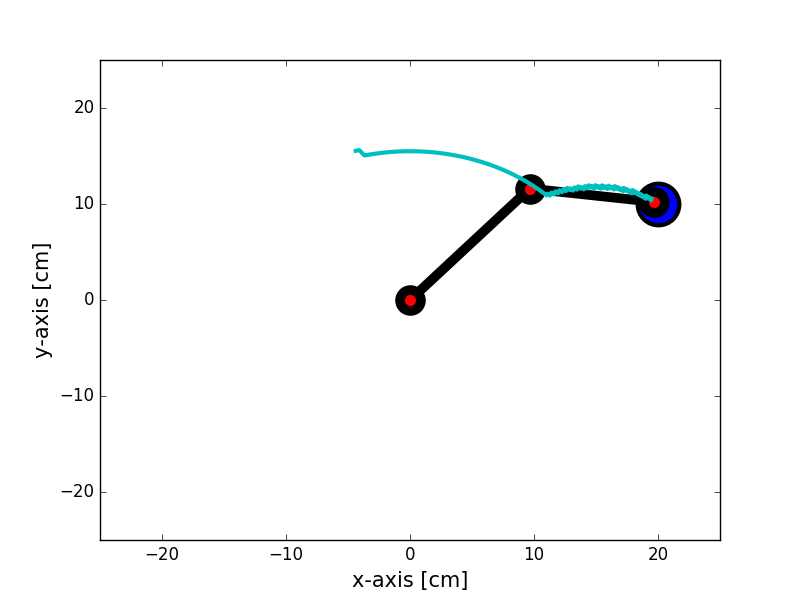
\includegraphics[width=.8\linewidth]{reportpics/scene1ik.png}
  \caption{Using IK}
  \label{fig:scenario1_ik}
\end{subfigure}%
\begin{subfigure}{.5\textwidth}
  \centering
  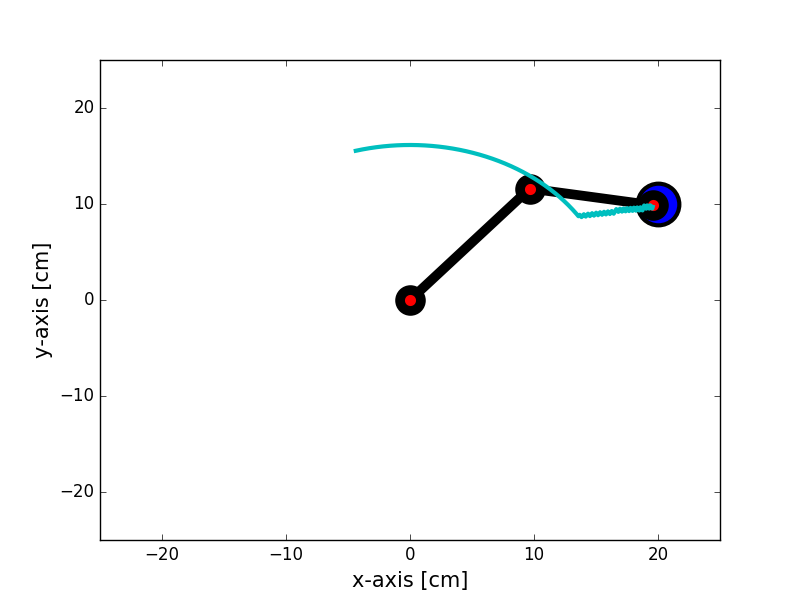
\includegraphics[width=.8\linewidth]{reportpics/scene1dqn.png}
  \caption{Using DQN}
  \label{fig:scenario1_dqn}
\end{subfigure}
\caption{Comparison between IK and DQN in $1^{rst}$ configuration}
\label{fig:scenario1}
\end{figure}

\begin{figure}[H]
\begin{subfigure}{.5\textwidth}
  \centering
  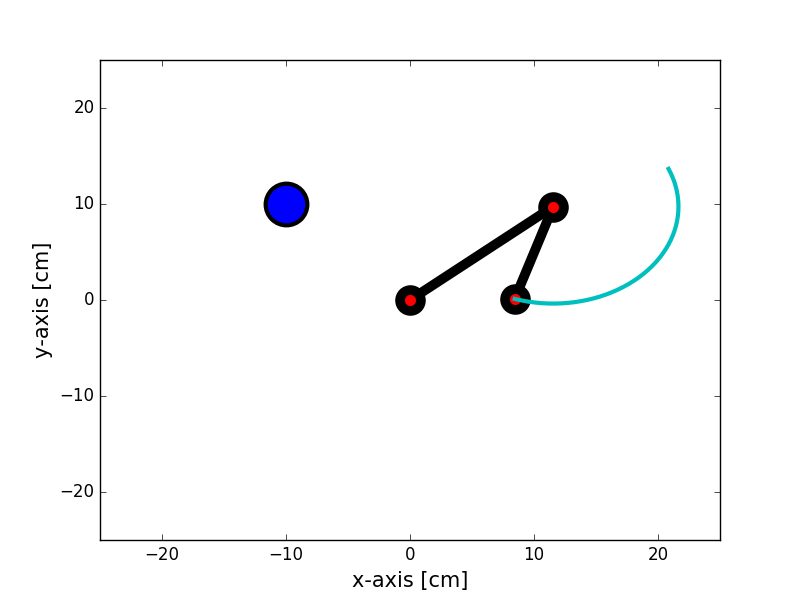
\includegraphics[width=.8\linewidth]{reportpics/scene2ik.png}
  \caption{Using IK}
  \label{fig:scenario2_ik}
\end{subfigure}%
\begin{subfigure}{.5\textwidth}
  \centering
  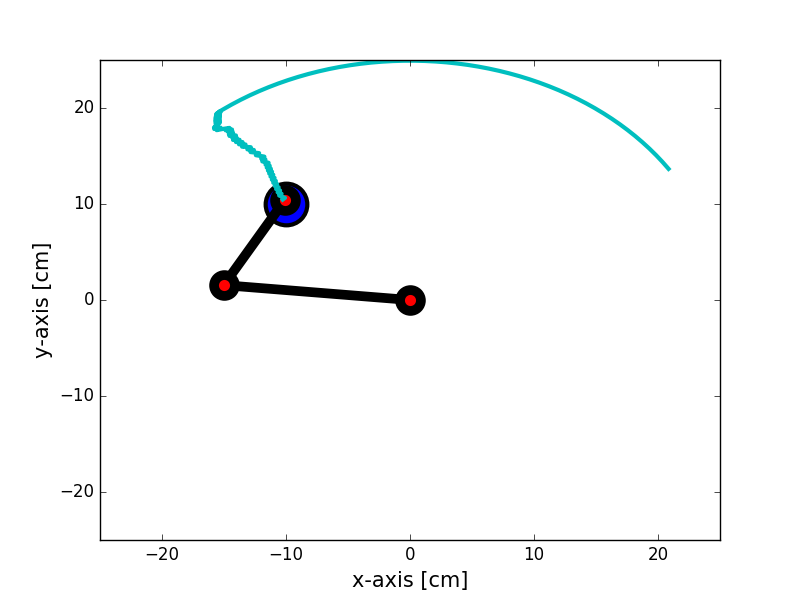
\includegraphics[width=.8\linewidth]{reportpics/scene2dqn.png}
  \caption{Using DQN}
  \label{fig:scenario2_dqn}
\end{subfigure}
\caption{Comparison between IK and DQN in $2^{nd}$ configuration}
\label{fig:scenario2}
\end{figure}

Testing the Q-Network also in the V-Rep simulation lead to the same results. This means that our approximations are not too severe and the Q-Network works also for the Poppy simulations and will be tested soon on the real robot.

\vspace{\baselineskip}

Finally, We plotted the $\max Q(s,a)$ as a function of the goal position to see if our neural network has actually learned a good approximation of the Q-function. With the reward function we chose, the Q-values should show concentric circles around the goal position, with decreasing the value the more the arm is far away from the goal. Exemplified in Fig.\ref{fig:maxQforTheta} the concentric circles can be indeed observed in this robot configuration as well as for other configurations.

\begin{figure}[H]
	\centering
	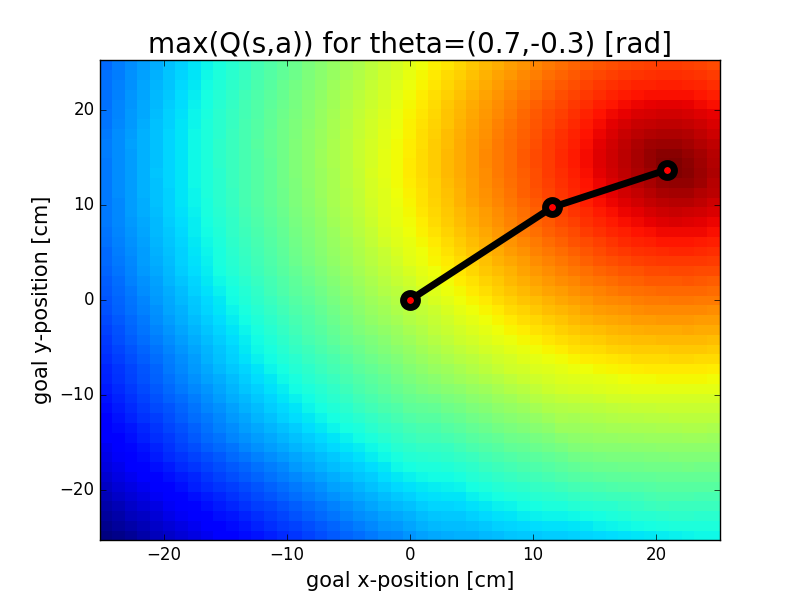
\includegraphics[width=0.7\textwidth]{reportpics/maxQforTheta.png}
	\caption{Plot of $\max Q(s,a)$ over different goal positions}
	\label{fig:maxQforTheta}
\end{figure}

\section{Milestones and Progress}
\begin{enumerate}
\item Set up the simulation (done)
\item Use the inverse kinematics as a base controller in simulation (done)
\item Use the inverse kinematics as a base controller on the robot (in progress)
\item Implement the DQN algorithm (done)
\item Include the simulation into DQN framework (done)
\item Train the Q-Network and tune hyper-parameters (done)
\item Try the Q-Network on the real robot (in progress)
\item Optional: vision for goal detection (in progress)
\item Optional: draw triangle or other shapes (not considered anymore)
\item Optional: use both arms (in progress)
\end{enumerate}

Taking the draft of project plan from the initial report, we achieved tuning of the hyper-parameters and training of good networks in the meantime. Testing on the Poppy robot is slowly advancing, but in progress, and we are trying to include optional milestones such as goal detection via vision and moving both arms. 
Taking into account the current progress of the project, we plan to complete our milestones as expected. 


%Therefore, we thought about new goals to achieve within the span of the project. Our current ideas are the following:
%\begin{itemize}
%\item Explore at which exact states in the state-space we do not have a proper description.
%\item Justify our parameters with empirical experiments.
%\item Graphical representation of the neural network (i.e. display the Q function).
%\end{itemize}


\newpage

\begin{thebibliography}{9}

%!!!!!!!!!!!!!!!!!!!!!!!!!!!!!!!!!!!!!!!!!!!!!!!!!!!!!!!!!!!!!!!!!!!!!!!!!!!!!!!!!!!!!%
%Pour la bibliographie, voilà la nouvelle manière de procéder pour faire les choses proprement :
%Ecrire dans la section "bibliographie" : \bibitem{nomDeLaRef} Auteur {\em Titre de la ref} date : lien vers le site ou éditeur du livre
%Ecrire à l'endroit où la référence est utilisée : \cite{nomDeLaRef}
%!!!!!!!!!!!!!!!!!!!!!!!!!!!!!!!!!!!!!!!!!!!!!!!!!!!!!!!!!!!!!!!!!!!!!!!!!!!!!!!!!!!!!%

%\bibitem{einstein} 
%Albert Einstein. 
%\textit{Zur Elektrodynamik bewegter K{\"o}rper}. (German) [\textit{On the electrodynamics of moving bodies}]. 
%Annalen der Physik, 322(10):891–921, 1905.




\bibitem{mnih_human} 
Volodymyr Mnih, Koray Kavukcuoglu, David Silver, Andrei A. Rusu, Joel Veness, Marc G. Bellemare, Alex Graves, Martin Riedmiller, Andreas K. Fidjeland, Georg Ostrovski, Stig Petersen, Charles Beattie, Amir Sadik, Ioannis Antonoglou, Helen King, Dharshan Kumaran, Daan Wierstra, Shane Legg
\& Demis Hassabis, Human-level control through deep reinforcement
learning, \textit{Nature}, \textit{doi:10.1038/nature14236}, 2015

\bibitem{mnih_play}
Volodymyr Mnih, Koray Kavukcuoglu   David Silver, Alex Graves, Ioannis Antonoglou, Daan Wierstra, Martin Riedmiller, Playing Atari with Deep Reinforcement Learning, \textit{DeepMind Technologies}, \textit{arXiv preprint arXiv:1312.5602}, 2013


\end{thebibliography}


\end{document}
